\chapter{Introduction}

Redaction is 'the act of removing words or information from a text before it is printed or made available to the public (Cambride Dictionary). Information or text is often redacted when it conveys sensitive information. This can be due to privacy and legal reasons, or because the text reflects the opinion of someone, or because of the risk of commercial conflicts from the publication of data. Multiple countries have \textit{Freedom of Information Acts} \cite{USAFia}, that require governmental bodies to release documents upon request of civilians. In The Netherlands the \textit{Wet open overheid (Woo)} \cite{WooWebsite} serves as such a law. This has resulted in different commercial text redaction tools in use by governments to speed up the redaction process. Different types of redacted text exist, from completely black filling (black-boxes) to gray bars to completely white, and even manual crossing out with a pen 
(\ref{fig:redactionExamples}).
\begin{figure}[h]
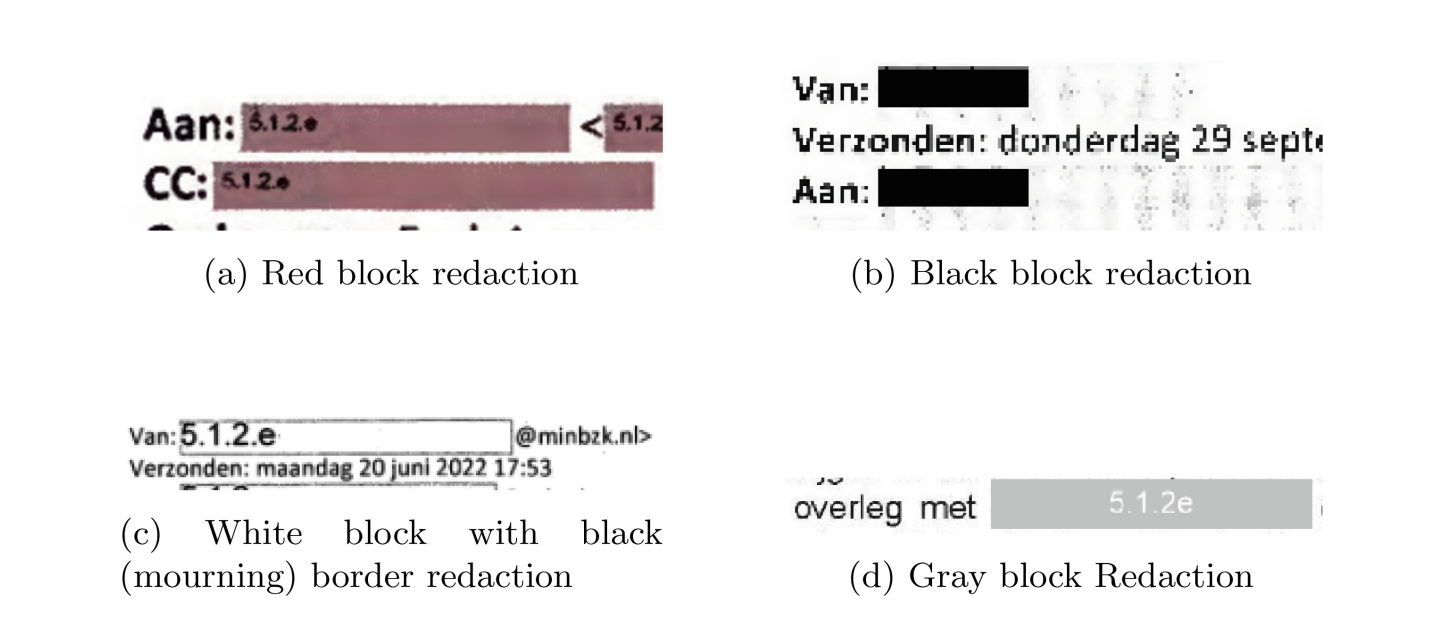
\includegraphics[width=\textwidth]{media/img.png}
\centering
\caption{Examples of four common types of text redactions. Codes like 5.1.2.e are inserted in the redacted regions to indicate the legal ground used to redact a particular piece of text.}
\label{fig:redactionExamples}
\end{figure}\\\\
Trivial redactions \cite{forrester2005investigation}, where text is obscured visually by the use of black boxes but the underlying content remains intact, often become the subject of ridicule and mockery. There are many examples of embarrassing redaction failures \cite{failures2019} that compromise the confidentiality of  sensitive information. Various tools have been developed to detect improper text redaction, such as the X-Ray Tool \cite{Xray2021}.
\\\\
Besides trivial redactions, other sensitive information may still be hidden in a document after processing or redaction \cite{muller2021processing}. Advanced features such as group editing, version control and multi-user authoring leave hidden information \cite{forrester2005investigation}; versions, track changes and metadata. 
\\\\
Two essential aspects are demanded of effective redaction. First, redaction has to \textit{really} remove sensitive information from a text or document. No sensitive information should be left in the rest of the document. Secondly, the information that does not have to be redacted has to be kept intact and visible for the reader. Governments and organisations often can not adhere to these two essential aspects of redaction. In many instances, the focus on safety is to the detriment of the non-redacted text which is damaged; more text is redacted or becomes unreadable. In the worst case all text is removed and only images of documents are made publicly available, especially when first scanning and then again OCR-ing documents is the predominant technique used by text-redaction tools. As a result, the accessibility is greatly damaged \cite{maartenMarx}. This is often the case in the Dutch text redaction landscape. 
\\\\
\begin{figure}[h]
    \begin{subfigure}[h]{0.5\linewidth}
        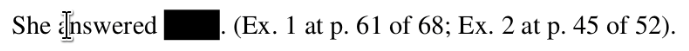
\includegraphics[width=\linewidth]{latex/media/badredaction2.png}
        \caption{A seemingly secure redaction.}
    \end{subfigure}
    \hfill
        \begin{subfigure}[h]{0.5\linewidth}
        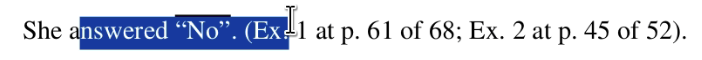
\includegraphics[width=\linewidth]{latex/media/badredaction.png}
    \caption{Selecting the box reveals the 'hidden' text.}
    \end{subfigure}%
\caption{An example of a bad redaction. The text has been 'redacted' by hiding it behind a black box. However, the actual text is not removed and hovering over it reveals the presence of the original text.}
\end{figure}
\\\\
I present a safe PDF redaction method for documents produced with Microsoft Word that ensures confidentiality of sensitive information and does preserve non-redacted text. Redaction is done directly in the PDF which is an advantage to redaction through first scanning a document and then OCR-ing it, preserving the text and accessibility. When applicable, my method inserts placeholder text and text on the same line as a redaction is repositioned. Furthermore, hidden information is either deleted or changed when possible. Finally, noise is added to positional information of glyphs in order to make it computationally difficult to determine what the original were. 
\\\\
By being able to account for all safety concerns, we are able to test our method using custom and real-world examples. Using tools such as X-ray, we were able to prove if our method was safe or not... \textbf{more to be added...}
\\\\
Our method performs... \textbf{more to be added...}


